\chapter{The ATLAS detector}
    \chapterprecishere{
        ``Potentielle citation sans aucun rapport avec le sujet"\par\raggedleft--- \textup{Personne inconnue}, contexte à déterminer
    }
    
   
        
    \section{General description and layout}
    
        \gls{atlas} experiment is a multipurpose detector at the \gls{lhc} built, along with its peer \gls{cms}, in order to probe the p-p, A-A and p-A collisions using the full \gls{lhc} luminosity \cite{atlas_experiment}. Being the largest (but not the heaviest) detector ever built for a collider experiment the \gls{atlas} detector comprises 44m in length, 25m in height and weights 7000 tonnes. \\
        The detector has a cylindrical shape and is an onion-like arrangement of several detector systems centered at the \gls{ip} as shown in fig. \ref{fig::atlas_layout}. The sub-detectors operate in the magnetic field created by the solenoid and toroid magnets (\gls{atlas} owes its name to the latter). Data acquisition and recording is controlled by the \gls{tdaq} systems, allowing eventually to lower the event rate to a value, acceptable for the data storage \cite{atlas_trigger}. The named systems are described in more detail in this chapter.
        
        
        \begin{figure}[htpb]
        		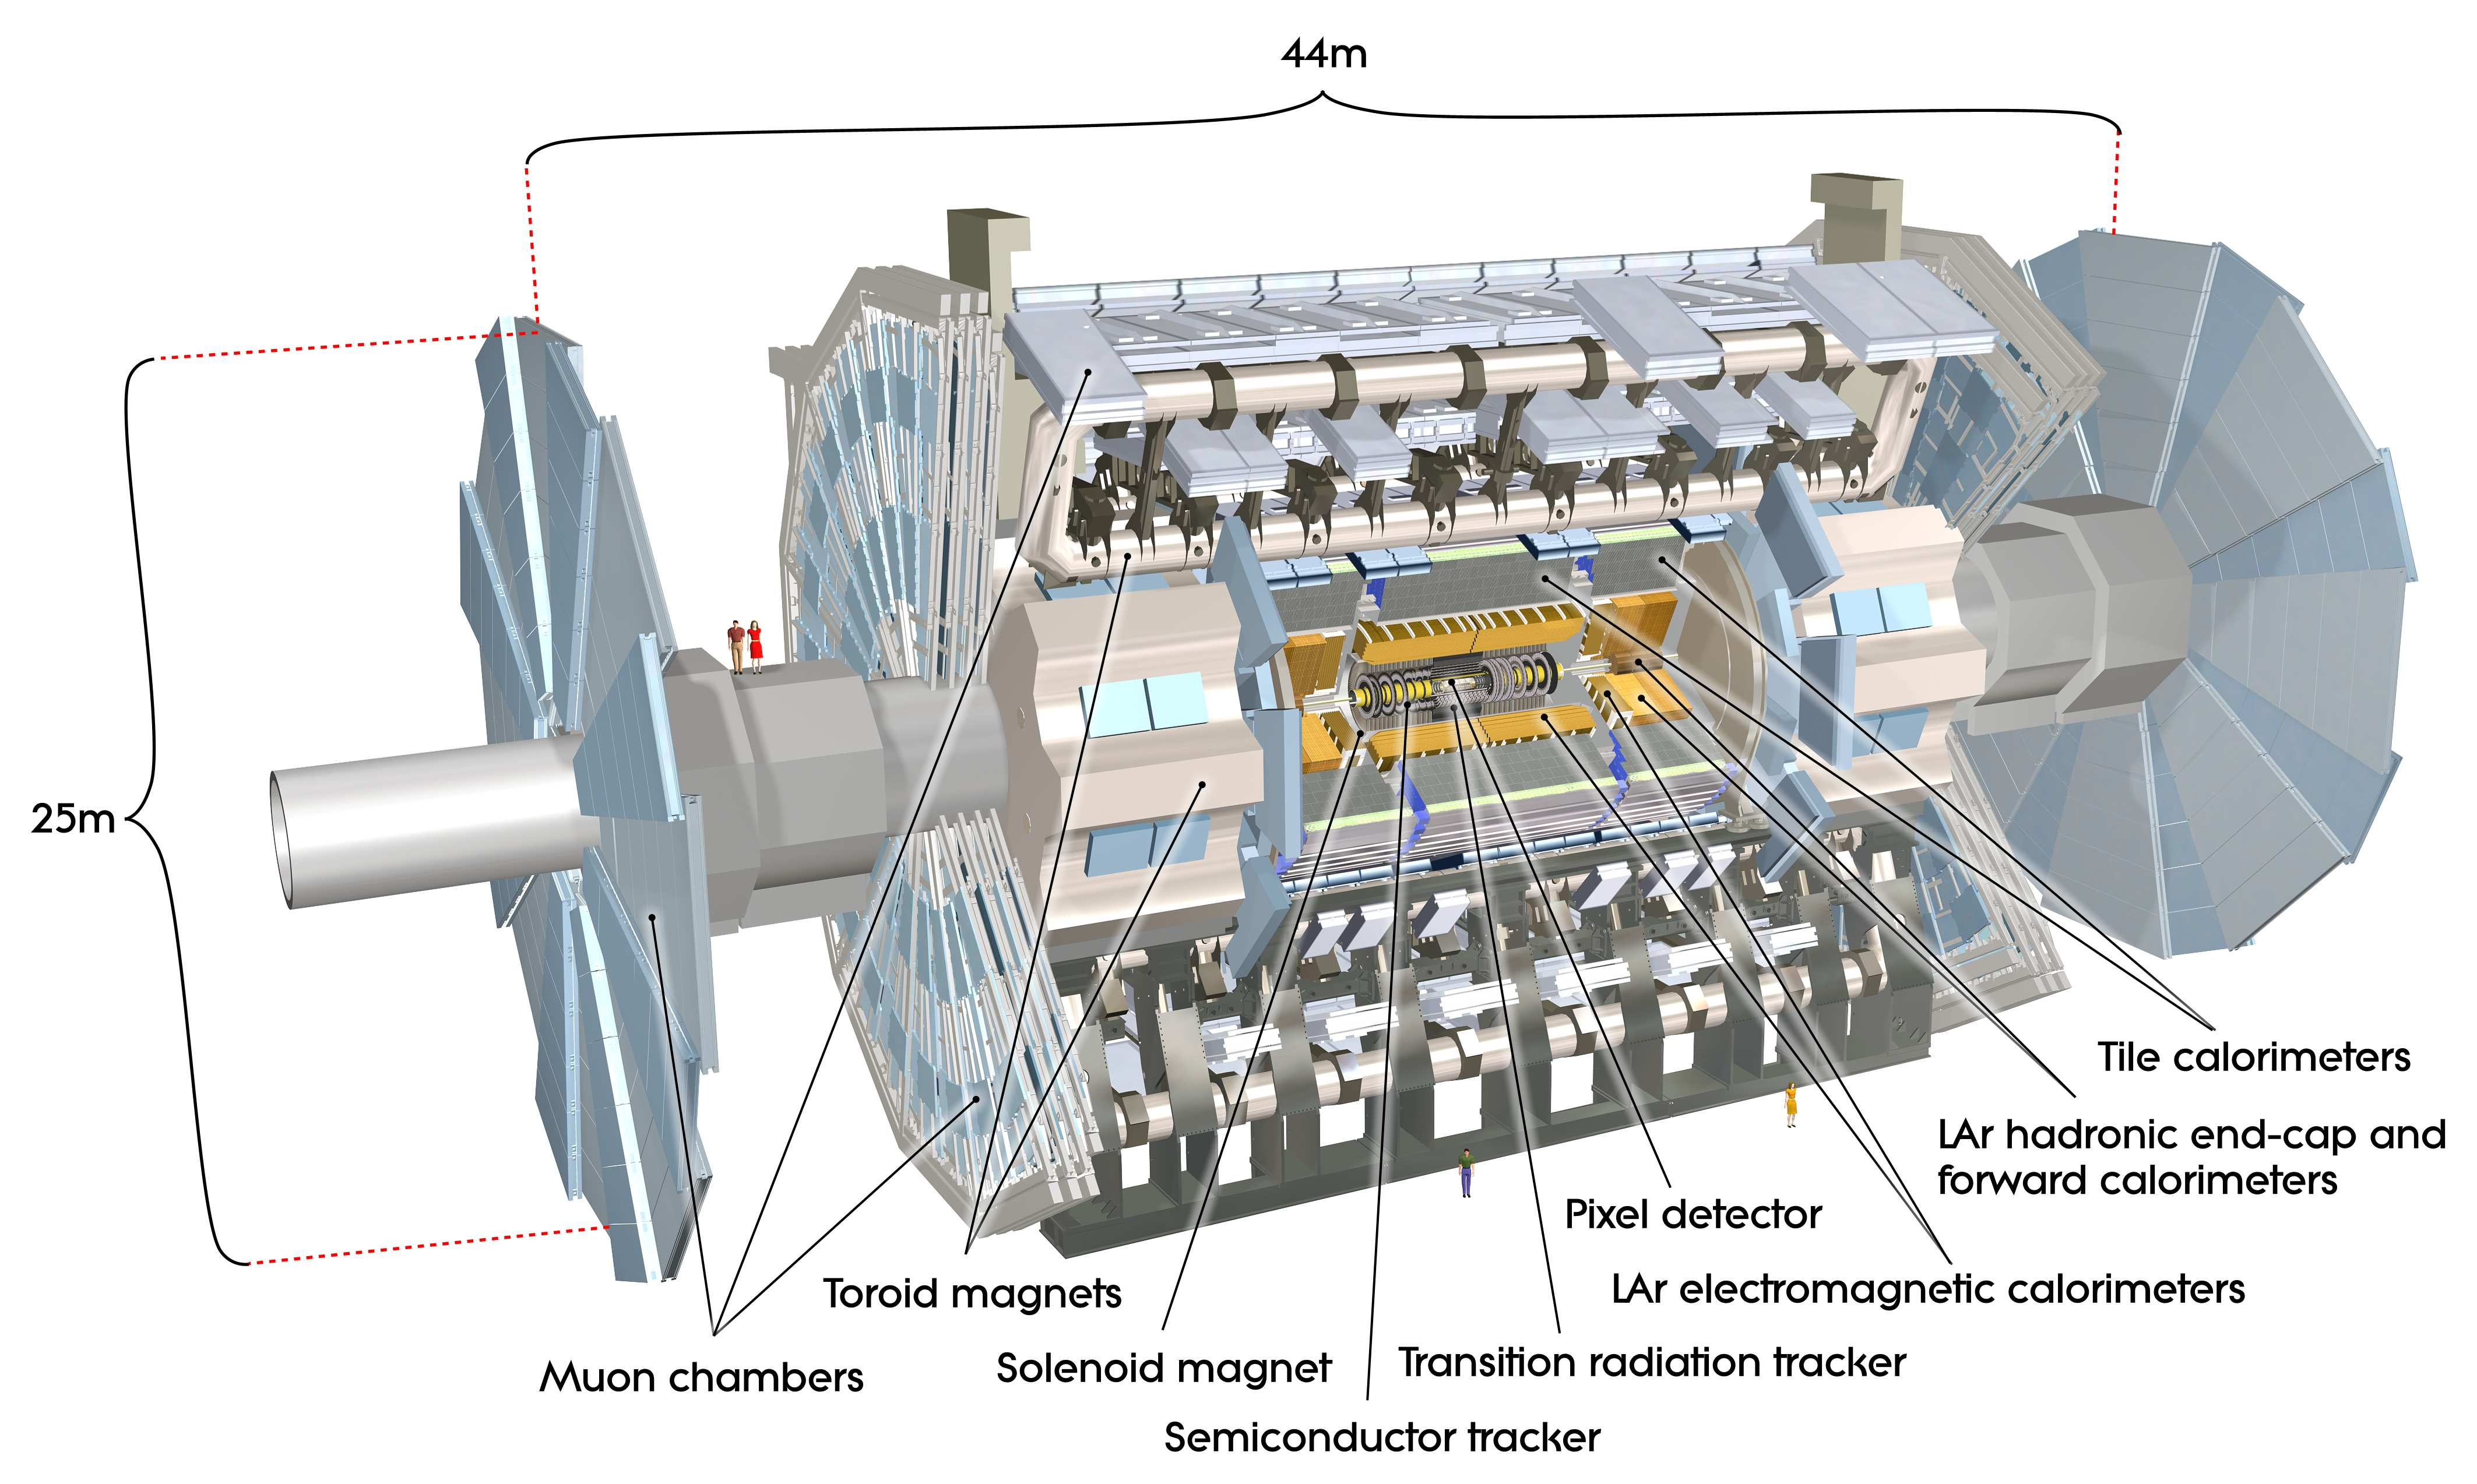
\includegraphics[width=\textwidth,keepaspectratio]{image--001.jpg}
        		\caption{ ATLAS detector general layout}
        		\label{fig::atlas_layout}
        \end{figure}
        
        \section{Coordinate system}
        
		The \gls{atlas} results often reference \gls{atlas} coordinates briefly described in this subsection. The origin of the right-handed coordinate system is placed at the \gls{ip} with \textit{z}-axis directed along the beam direction. This, in turn, defines the transverse \textit{x-y} plane with $\textit{x}$ axis pointing towards the center of the \gls{lhc} ring and \textit{y} axis directed upwards. All transverse observables like $p_T$ and $E_T$ are defined in this 2D plane. Besides the mentioned Carthesian coordinates the asimuthal angle \textit{$\phi$} is defined in the transverse plane around the beam axis. Polar angle \textit{$\theta$} is the elevation angle measured from the beam axis. The following metric quantities are also to be mentioned:
		\begin{itemize}
		\item Pseudorapidity $\eta$ = -ln tan($\theta$/2),
		\item Rapidity $y$ = 1/2 ln [(E+$p_z$)/(E-$p_z$)]
		\item The distance between particles $\Delta R = \sqrt{\Delta \eta^2 + \Delta \phi ^2}$
		\end{itemize}
        
        \section{Magnet system and magnetic field}\label{atlas_magnets}
        \gls{atlas} has a hybrid system of four supercoducting magnets which has 22 m in diameter, 26 m in length and stores an energy of 1.6 GJ \cite{magnet_tdr1}. The windings of the magnets are schematically shown in fig. \ref{fig::atlas_magnets}. The four magnets that comprise the magnet system are the following: 
        		\begin{itemize}
        	\item The central solenoid is aligned with the beam axis providing 2T axial magnetic field for the inner detector.
        	\item A barrel toroid produces toroidal magnetic field of about 0.5T for the muon detectors in the barrel region.
        	\item Two end-cap toroids produce toroidal magnetic field of approximately 1T for the muon detectors in the end-cap regions.
        \end{itemize}
        \begin{figure}[htpb]
        	\centering
        	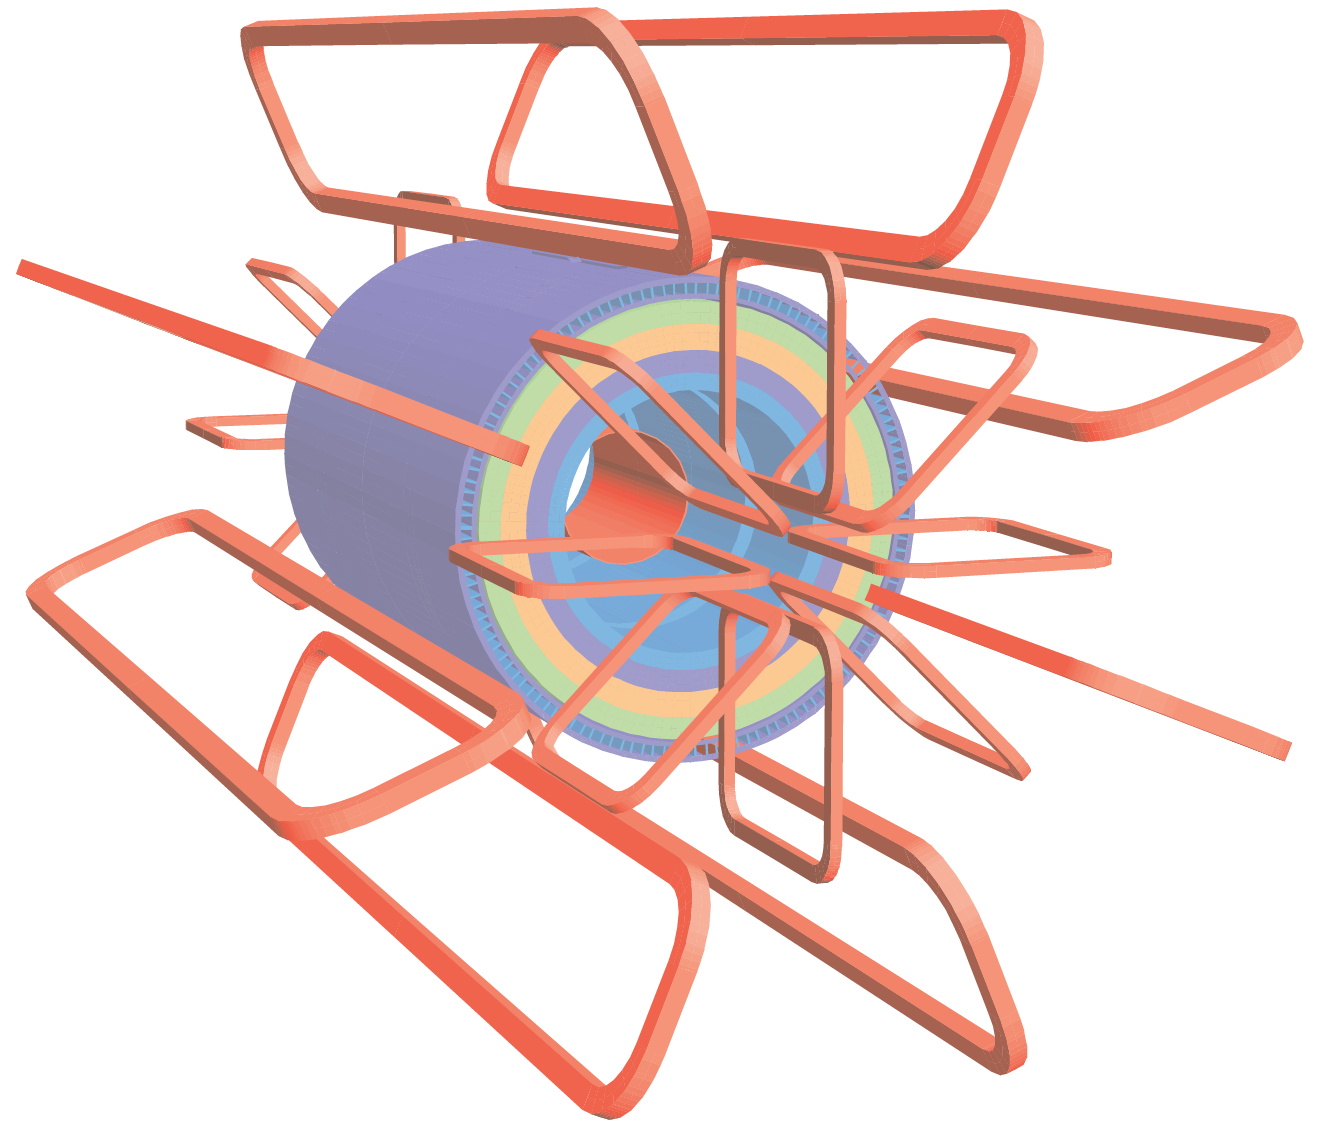
\includegraphics[width=0.7\textwidth,keepaspectratio]{magnets_scheme.png}
        	\caption{Geometry of \gls{atlas} magnet windings}
        	\label{fig::atlas_magnets}
        \end{figure}
        \section{Inner detector}
		The \gls{atlas} \gls{id} is designed to deliver pattern recognition, high-resolution momentum measurement \cite{id_tdr1},\cite{id_tdr2} along with primary and secondary vertex determination for charged particle tracks above a designated $p_T$ threshold of 0.5 GeV (in some cases being capable of going as low as 0.1 GeV) within the pseudorapidity range $|\eta| < 2.5$. The inner detector provides reliable electron identification in rapidity range of $|\eta| < 2.0$ for energies from 0.5 GeV to 150 GeV.\\
		The  \gls{id} layout is a result of the technical requirements: it is assembled in a cylindrical envelope of 3512 mm in length and 1150 mm in radius. It is surrounded by the magnetic field of 2T imposed by the superconducting solenoid (see section \ref{atlas_magnets}).\\
		Three independent sub-detectors complement each other in the inner detector (see fig. \ref{fig::id} (a)):
		\begin{itemize}
		\item Silicon pixel with 3 cylindrical layers for the barrel and 3 discs on each side for the end-cap. It provides the highest granularity around the vertex region. Normally each track hits three pixel layers. The pixel detector has about 80.4 million readout channels. Each of 1744 identical pixel sensors has 47232 pixels and 46080 readout channels. About 90\% of the pixels have the size of 50x400 $\mu m^2$, the remaining pixels are a bit longer: 50x600 $\mu m^2$.
		\item Silicon microstrip layers (SCT) with 4 cylindrical layers and 9 discs on each side for the end-cap. A track typically crosses the strip layers in four space points. SCT has approximately 6.3 millions readout channels from its 15912 sensors. There are 768 active stripts of 12 cm lenght and 80 $\mu$m width per sensor plus two bias potential strips on the sensor edges.
		\item Transition radiation tracker (TRT) with 73 straw planes in the barrel and 160 straw planes in the end-cap. The TRT has around 351,000 readout channels and detects in average 36 hits per track. The straw tubes that make up the TRT module are 4 mm thick and 1.44 m long (0.37 m in the endcap) and made out of polyamide films reinforced with carbon fibers. The straws are filled with gas mixture of 70\% Xe, 27\% CO$_2$ and 3\%O$_2$ and supplied with gilded tungsten anodes which are directly connected to the readout channels.
		The pixel and SCT sensors are highly radiation-proof and operate in the temperature range from -5$^\circ$C to -10$^\circ$C to minimize the radiation damage, while the TRT module operates at room temperature.	
		\end{itemize}
		\begin{figure}[htbp]
			\begin{subfigure}[t]{0.48\textwidth}
				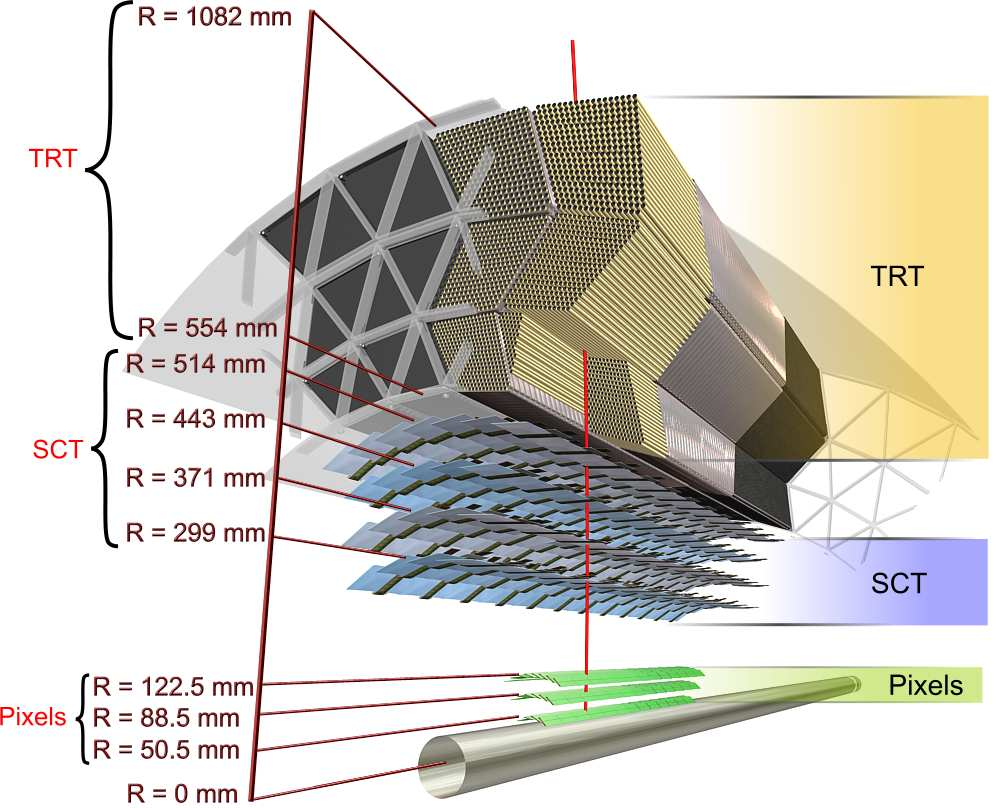
\includegraphics[width=\textwidth,keepaspectratio]{image--076.jpg}
				\caption[Inner detector]{Inner detector}
				\label{fig::id}
			\end{subfigure}
		                \hfill
			\begin{subfigure}[t]{0.48\textwidth}
				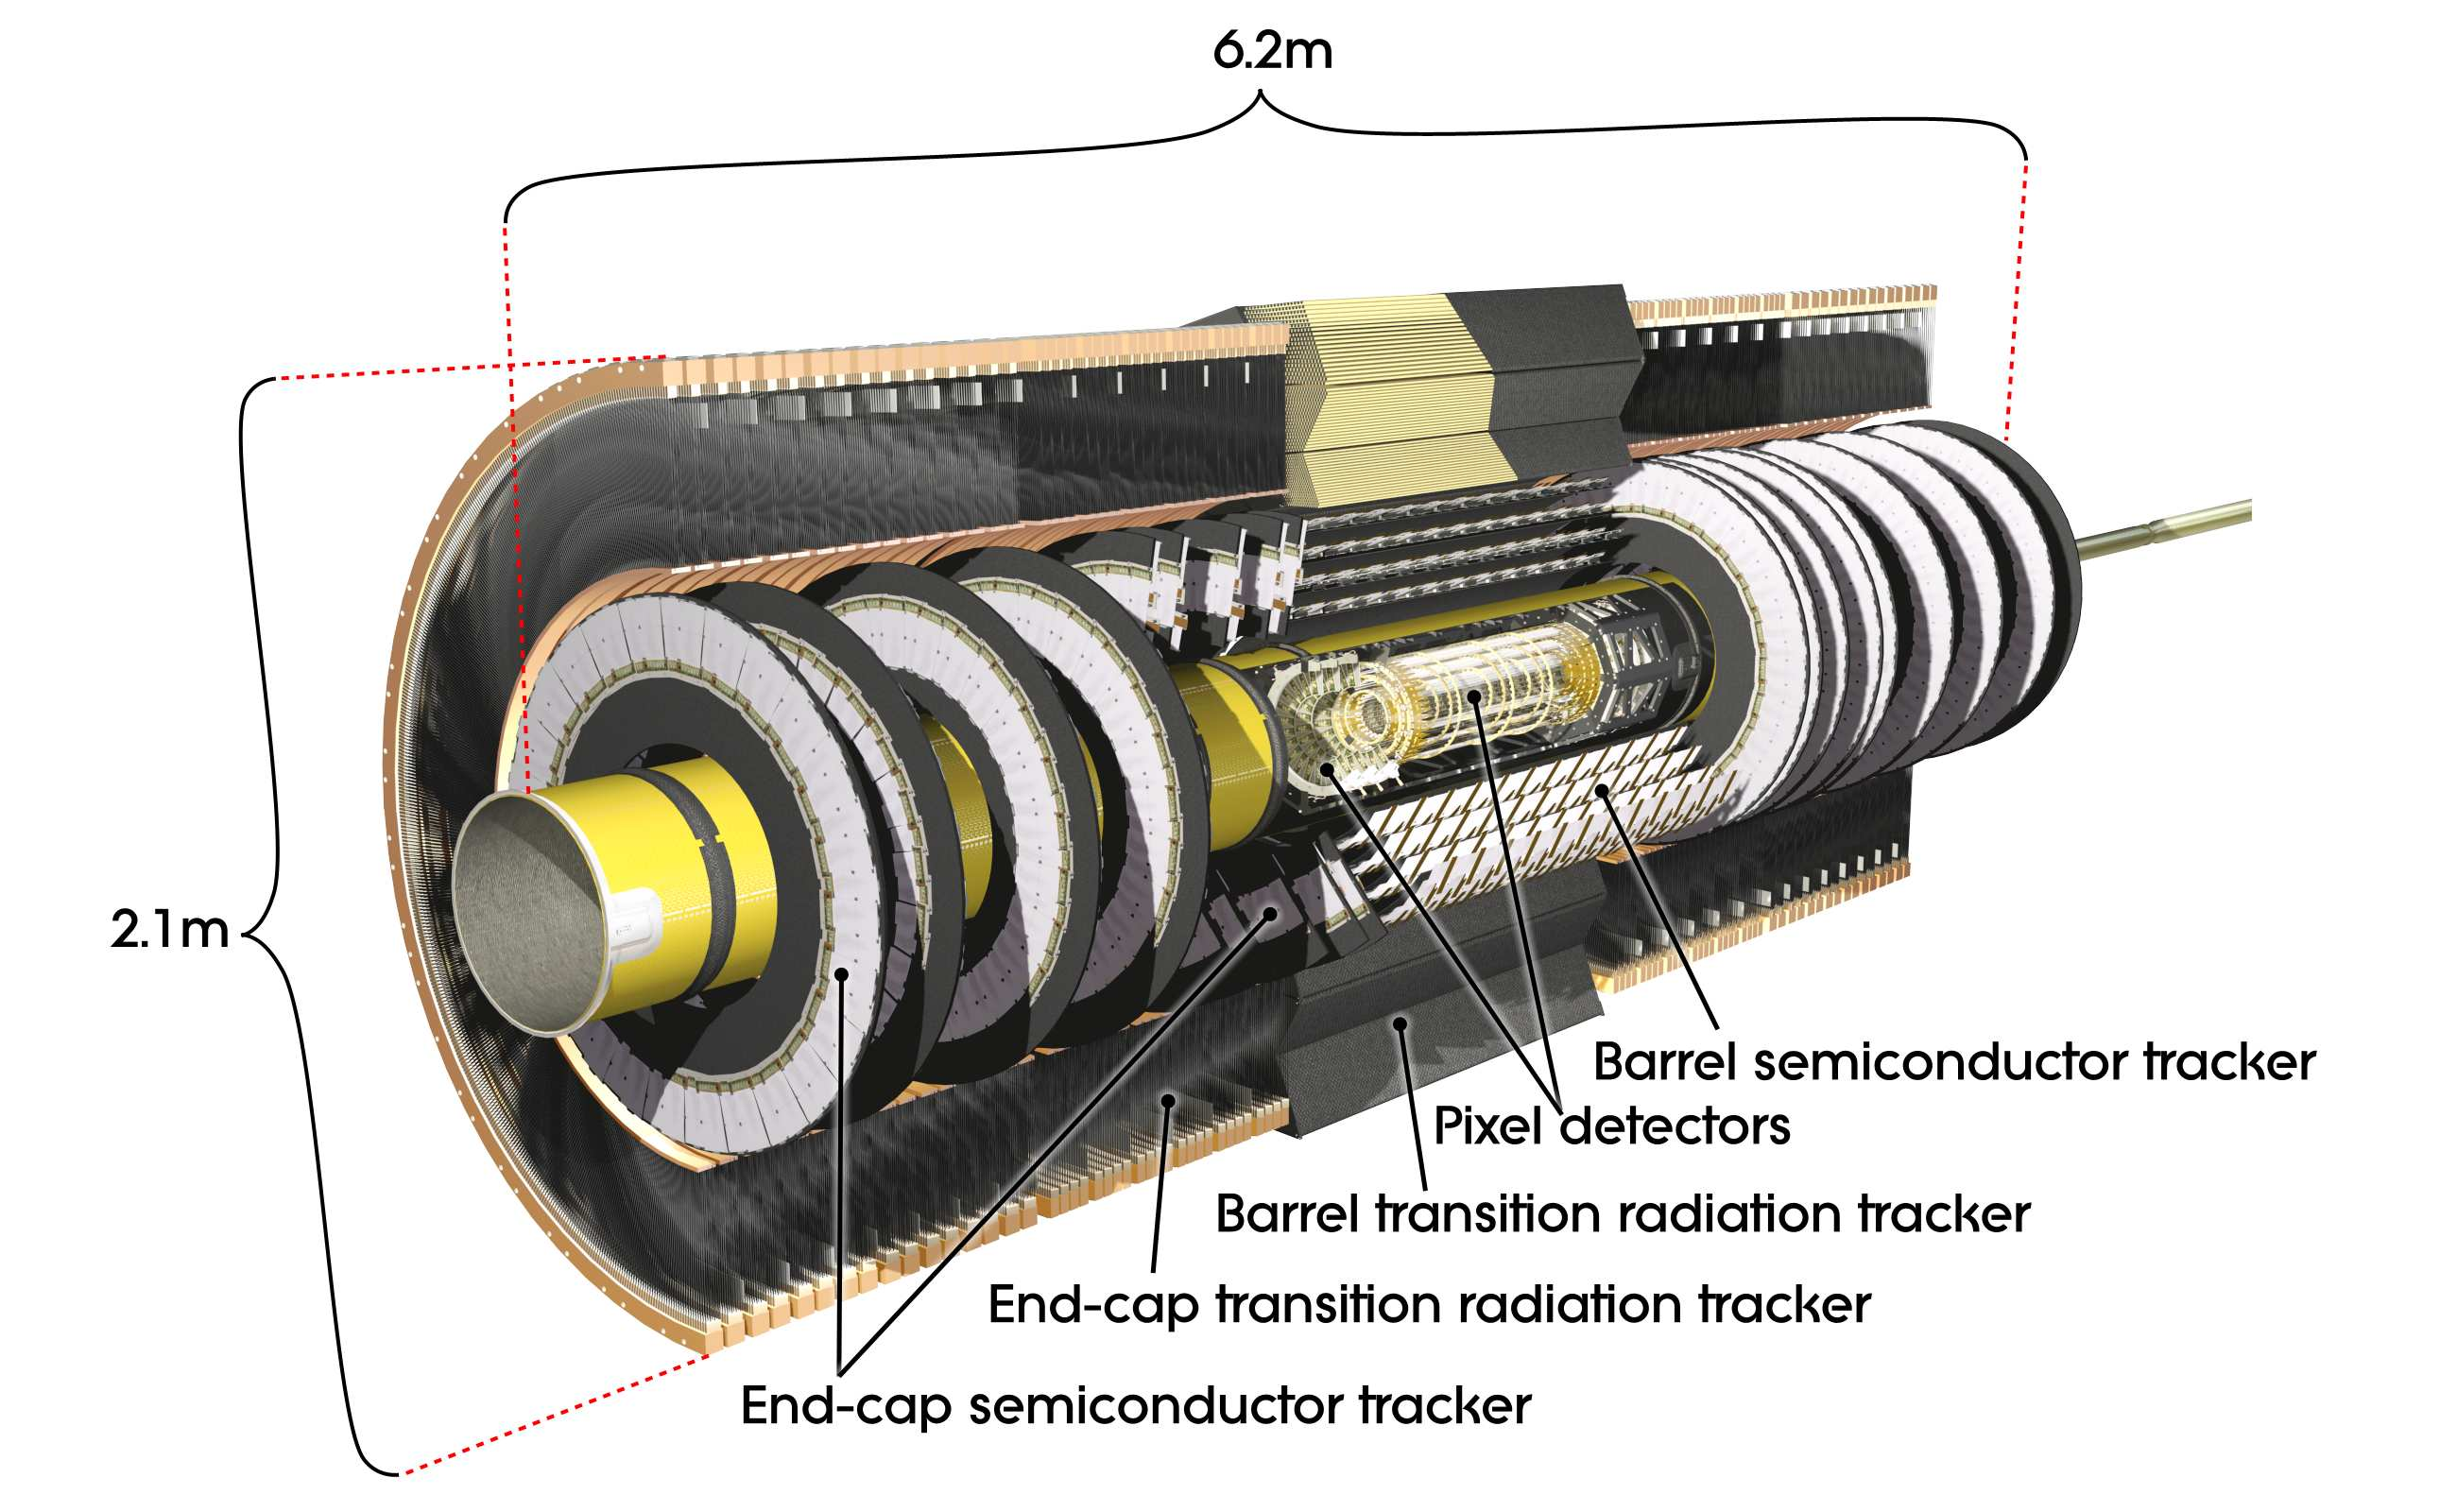
\includegraphics[width=\textwidth,keepaspectratio]{image--002.jpg}
				\caption[Pixel detector]{A perspective cut-away view of the pixel detector.}
				\label{fig::pd}
			\end{subfigure}
			\caption{Fichier Gerber des modèles d CFR-34 et CFR-35.}
			\label{fig::cfrs}
		\end{figure}
        \section{Calorimeter system }
		The ATLAS calorimeter system covers the rapidity range within $|\eta| < 4.9$ and consists of several different detector systems. A rapidity region matched to the inner detector posesses fine granularity perfectly suited for high-precision measurements of photons and electrons. The remaining part's granularity is coarser but enough to perform jet reconstruction and measure $E_T^{miss}$. The view of ATLAS calorimeter is presented on fig. \ref{fig::calorimeter_layout}.\\
		Besides measuring the energy of travelling particles calorimeters must also contain electromagnetic and hadronic showers, limiting their ability to go penetrate the calorimeter completely and get to the muon chambers. This provides a typical scale for size of the calorimeter modules: the EM calorimeter\cite{LAr_calo} is >22 radiation lengths ($X_0$) in the barrel and >24$X_0$ in the end-caps. The hadronic calorimeter has the thickness of 9.7 interaction lengths ($\lambda$) in the barrel and 10$\lambda$of in the endcap, which is enough to keep the leakage level below the typical muon background. This size also provides good resolution for the $E_T^{miss}$ measuremet. The detailed description of the calorimeter system can be found in the table \ref{tab::calorimeter_table}.
		The tile calorimeter\cite{Tile_calo} uses scintillating tiles as active material alternated with steel absorbers. All the other calorimeter systems use liquid argon as an active medium with lead sampling.
        \begin{figure}[htpb]
			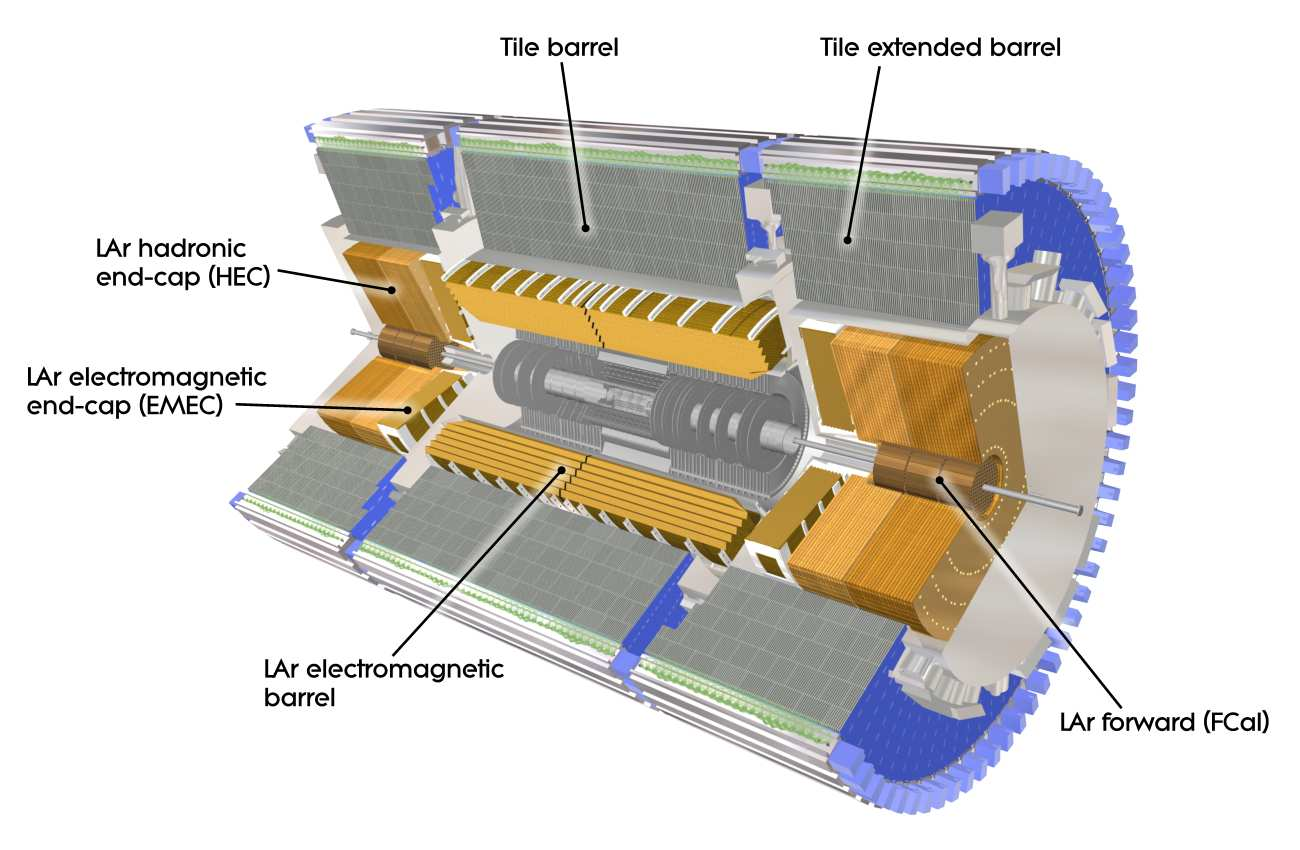
\includegraphics[width=\textwidth,keepaspectratio]{image--003.jpg}
			\caption{ \gls{atlas} calorimeter general layout}
			\label{fig::calorimeter_layout}
		\end{figure}
	\begin{table}
		\centering
		\begin{tabular}{|c|l r| l r|}
			\hline
		     &
			 \multicolumn{2}{|c|}{ Barrel} &
			\multicolumn{2}{|c|}{ End-cap} \\
			\hline
		   \multicolumn{5}{|c|}{\textbf{EM Calorimeter}} \\
			\hline			
			\multicolumn{5}{|c|}{Number of layers and $|\eta|$ coverage} \\
			\hline			
			Presampler & 1 &$|\eta|$  <1.52  & 1 & 1.5 < $|\eta|$  <1.8\\
			\hline
			Calorimeter& 3 &$|\eta|$  <1.35  & 2 & 1.375 < $|\eta|$  <1.5\\
			\hline
			\multicolumn{5}{|c|}{Granularity $\Delta \eta x \Delta \phi$ versus $|\eta|$} \\
			\hline
			Presampler& 0.025$\times$0.1 &$|\eta|$  <1.52  & 0.025$\times$0.1 & 1.5 < $|\eta|$  <1.8\\
			\hline
			Calorimeter 1st layer& 0.025/8$\times$0.1 &$|\eta|$  <1.40  & 0.050$\times$0.1 & 1.375 < $|\eta|$  <1.425\\
			& 0.025$\times$0.025 &1.425 < $|\eta|$  <1.5  & 0.025$\times$0.1 & 1.425 < $|\eta|$  <1.5\\
			&  &  & 0.025/8$\times$0.1 & 1.5 < $|\eta|$  <1.8\\
			&  &  & 0.025/6$\times$0.1 & 1.8 < $|\eta|$  <2.0\\
			&  &  & 0.025/4$\times$0.1 & 2.0 < $|\eta|$  <2.4\\
			&  &  & 0.025$\times$0.1 & 2.4 < $|\eta|$  <2.5\\
			&  &  & 0.1$\times$0.1 & 2.5 < $|\eta|$  <3.2\\
			\hline
			Calorimeter 2nd layer& 0.025$\times$0.025 &$|\eta|$  <1.40  & 0.050$\times$0.1 & 1.375 < $|\eta|$  <1.425\\
			& 0.075$\times$0.025 &1.4 < $|\eta|$  <1.475  & 0.025$\times$0.025 & 1.425 < $|\eta|$  <2.5\\
			&  &  & 0.1$\times$0.1 & 2.5 < $|\eta|$  <3.2\\
			\hline
			Calorimeter 3rd layer& 0.050$\times$0.025 &$|\eta|$  <1.35  & 0.050$\times$0.025 & 1.5 < $|\eta|$  <2.5\\
			\hline
			\multicolumn{5}{|c|}{Number of readout channels} \\
			\hline
			Presampler& 7808& & 1536 (both sides) & \\
			Calorimeter& 101760& &62208 (both sides) & \\
			\hline	
			\multicolumn{5}{|c|}{\textbf{LAr hadronic end-cap}} \\
			\hline
			$|\eta|$  coverage &  &  & 1.5 < $|\eta|$  <3.2 & \\
			Number of layers &  &  & 4 & \\
			\hline
			Granularity $\Delta \eta \times \Delta \phi$ &  & 0.1 $\times$ 0.1 & 1.5 < $|\eta|$  <2.5 & \\
			 &  & 0.2 $\times$ 0.2 & 2.5 < $|\eta|$  <3.2 & \\
			\hline
			Readout channels&  &  &5632 (both sides)\\
			\hline	
			\multicolumn{5}{|c|}{\textbf{LAr forward calorimeter}} \\
			\hline
			$|\eta|$  coverage &  &  & 3.1 < $|\eta|$  <4.9 & \\
			Number of layers &  &  & 3 & \\
			\hline
			Granularity $\Delta x \times \Delta y$ &  & & FCal 3.0 $\times$ 2.6 & 3.15 < $|\eta|$  <4.30  	\\
			&  & &FCal: $\sim$four times finer & 3.10 < $|\eta|$  <3.15  \\
			&  &  & & 4.30 < $|\eta|$  < 4.83  \\
			&  & & FCal2 3.3 $\times$ 4.2 & 3.24 < $|\eta|$  <4.50  \\			
			&  & & FCal2: $\sim$four times finer & 3.20 < $|\eta|$  <3.24 \\
			&  &  & & 4.50 < $|\eta|$  < 4.81 \\
			&  & & FCal3 5.4 $\times$ 4.7 & 3.32 < $|\eta|$  <4.60 \\			
			&  & & FCal3: $\sim$four times finer & 3.29 < $|\eta|$  <3.32  \\
			&  &  & & 4.60 < $|\eta|$  < 4.75  \\
			\hline
			Readout channels&  &  &3524 (both sides)\\
			\hline	
			\multicolumn{5}{|c|}{\textbf{Scintillator tile calorimeter}} \\
			\hline
			& \multicolumn{2}{|c|}{ Barrel} & \multicolumn{2}{|c|}{ Extended barel} \\
			\hline
			$|\eta|$  coverage & $|\eta|$  < 1.0 &  & 0.8 < $|\eta|$  <1.7 & \\
			Number of layers &  3 &  & 3 & \\
			\hline
			Granularity $\Delta \eta \times \Delta \phi$ &  & 0.1 $\times$ 0.1 & 0.1 $\times$ 0.1  & \\
			&  & 0.2 $\times$ 0.2 & 0.2 $\times$ 0.1  & \\
			\hline
			Readout channels&  5760 &  &4092 (both sides)\\
			\hline	
	\end{tabular}\\
	\caption{ \gls{atlas} calorimeter in numbers}
	\label{tab::calorimeter_table}
\end{table}
	
	
	
        \subsection{Electromagnetic calorimeter }
        \label{emc}
        The \gls{emc} has two submodules:
        \begin{itemize}
        	\item \gls{emc} barrel detector.
        	\item \gls{emec} end-cap detector.
        \end{itemize}
        The \gls{emc} barrel module consists of two identical half-barrels 3.2 meters long with inner and outer radii 2.8 m and 4 m respectively. There is a 4mm gap at $z$ = 0 between the half-barrels. The second crack is situated between the barrel and the end-cap at $1.37 < |\eta| < 1.52$. The \gls{emec} comprises of two pairs of coaxial wheels of 63 cm thick having inner and outer radii of 330 mm and 2098 mm respectively. The crack between the two wheels makes a third crack at  $|\eta| = 2.5$.
        Both barrel and end-cap electromagnetic calorimeters are designed to have an accordion-shaped absorbers made out of lead plates, coated in stainless steel sheets. The readout electrodes are placed in the gaps between the absorbers. This type of geometry allows full coverage in $\phi$ without cracks together with fast extraction of the signal from both sides of the electrodes. The orientation of the accordion waves is axial in the barrel and radial in the end-caps (see fig. \ref{fig::calorimeter_layout}). These features of the calorimeter lead to virtually uniform performace in $\phi$ dimension. \\
        Segmentation in $\eta$  is very different in the layers of the calorimeter, but the second layer always has the finest granularity because the egamma particles are supposed to leave most of their energy in the second calorimeter layer. In order to correct for the energy losses upstream the barrel calorimeter is preceded by a thin LAr active layer of  11mm thick called a presampler. For more details on $\eta$ coverage and granularity see table \ref{tab::calorimeter_table}.

        \begin{figure}[htpb]
        	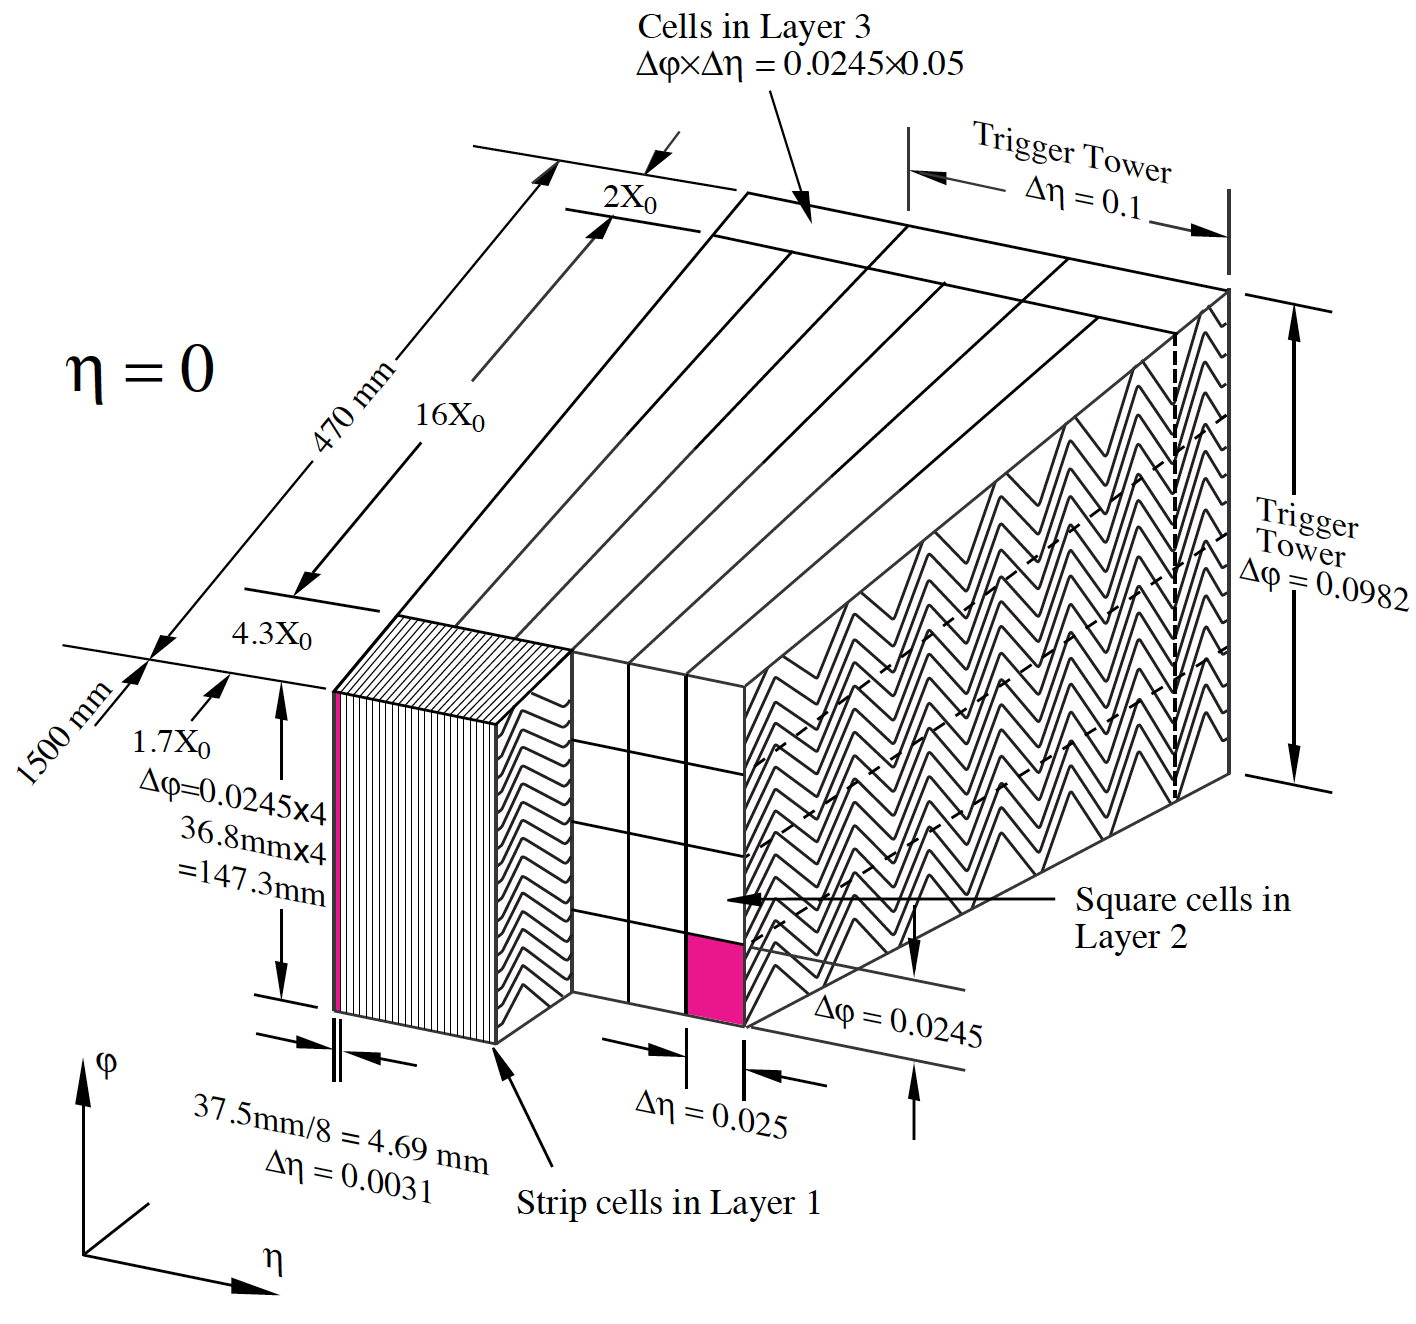
\includegraphics[width=\textwidth,keepaspectratio]{EMcalo_layers.png}
        	\caption{ \gls{atlas} EM calorimeter layers}
        	\label{fig::calorimeter_layers}
        \end{figure}
    
        \begin{figure}[htbp]
        			\begin{subfigure}[t]{0.48\textwidth}
        				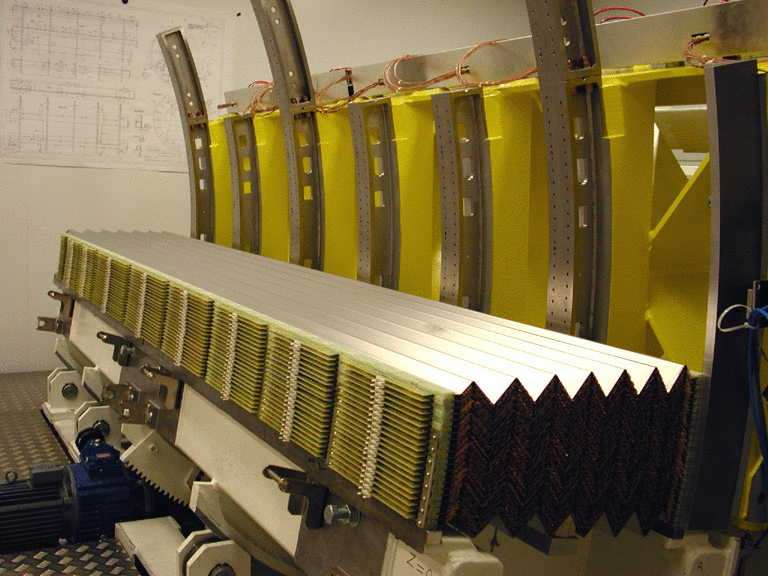
\includegraphics[width=\textwidth,keepaspectratio]{image--112.jpg}
        				\caption[Barrel]{Barrel}
        				\label{fig::barrel}
		\end{subfigure}
        		                \hfill
        \begin{subfigure}[t]{0.48\textwidth} 
				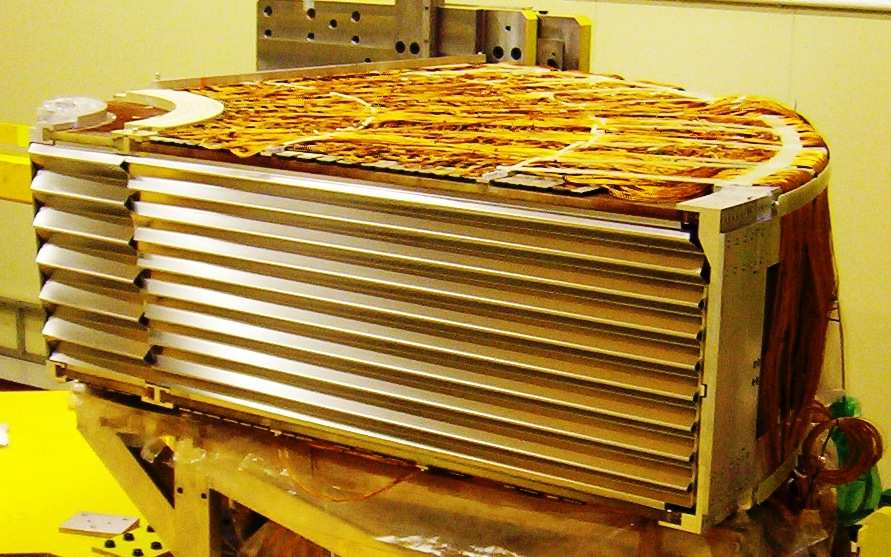
\includegraphics[width=\textwidth,keepaspectratio]{image--113.jpg}
				\caption[End-cap]{End-cap}
				\label{fig::endcap}
		\end{subfigure}
			\caption{Accordion absorbers of the \gls{emc}}
			\label{fig::accordion}
		\end{figure}
	\subsection{Hadronic calorimeter }
	        The \gls{hc} is combined of three submodules:
	\begin{itemize}
		\item \gls{hc} scintilating tile detector, a steel sampled detector divided in turn into central barrel having 5.8 m in length and two extended barrels 2.6 m in length each. The extended barrels have inner radii of 2.28 m and outer radii of 4.25 m.  The tile calorimeter consists of three layers having about 1.5, 4.1 and 1.8 interaction lengths $\lambda$ in the barrel and 1.5, 2.6 and 3.3 $\lambda$s in the extended barrel. 
		\item \gls{hec} detector is a liquid argon calorimeter sampled with copper. It has two pairs of independent wheels symmetrically located behind the \gls{emec} called the frona and the rear wheel. The wheels are cylindrical, their outer radius is 2030mm. 
		\item \gls{fcal} detector modules are located about 4.7 m from the \gls{ip} and are subjected to very high particle flux and radiation. It consists of three wheels 45 cm deep each. The first one, FCal1 is sampled with copper intended for the measurement of electromagnetic processes. The two other wheels FCal2 and FCal3 are sampled with tungsted and designed for the hadronic showers measurement.
	\end{itemize}
	The number of the readout channels as well as the $\eta$ coverage of every module and submodule is described in the Table \ref{tab::calorimeter_table}.
	
\section{Muon detectors}
\label{sect::muons}
    \begin{figure}[htpb]
	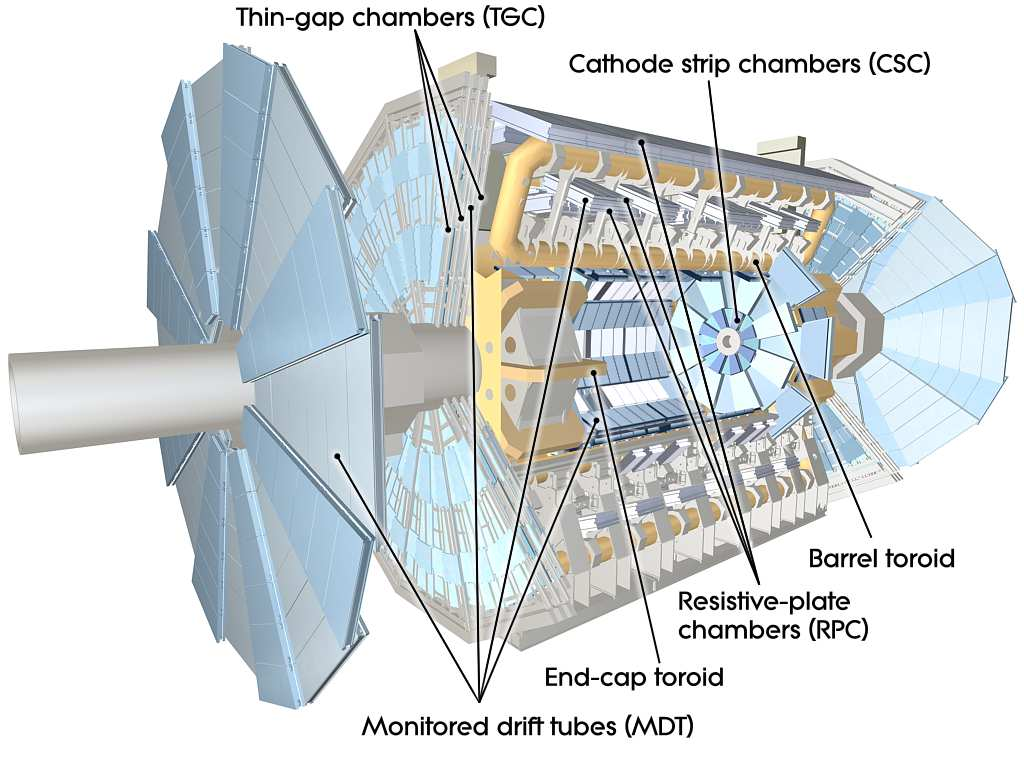
\includegraphics[width=\textwidth,keepaspectratio]{image--004.jpg}
	\caption{ \gls{atlas} muon system}
	\label{fig::muon_layout}
	\end{figure}

	Most of the muons produced as a result of the p-p collisions are able to penetrate through calorimeters and make it to the muon detectors where their tracks are getting measured. The spectrometer provides high-precision measurement of the muon momenta in the rapidity range of $|\eta| < 2.7$ and approximate transverse momentum range of 3 GeV < $p_T$ < 3 TeV. The lower bound on the momentum is mainly due to energy losses in the calorimeter, while the upper bound is caused by the saggita bias coming from the tracking chambers alignment. The goal $p_T$ resolution is about 10\% for a 1 TeV muon track. \\
	The muon tracks\cite{muons_1},\cite{muons_2}  are bent by the torroid magnets allowing to determine muon kinematic properties. The large barrel toroid covers the rapidity range of $|\eta| < 1.4$, while at  $1.6 < |\eta| < 2.7$ the tracks are bent by the smaller end-cap magnets. The deflection in the transition region of $1.4 < |\eta| < 1.6$ is provided by the barrel and end-cap fields combined.\\
	The general layout of the muon spectrometer is depicted on fig. \ref{fig::muon_layout}, the parameters of the muon systems can be found in table \ref{fig::muon_table}. Just like the rest of the detector systems the muon spectrometer is split into the barrel and the end-cap parts. \\ 
	The muon spectrometer possesses a fast triggering system able to trigger for muons in the rapidity range of $|\eta| < 2.4$. It delivers the track information within a few tens of nanoseconds after the particle passage which also allows to use it for the bunch-crossing identification. The trigger chambers measure both $\eta$ and $\phi$ coordinates of a track of which the former is in the bending plane and the latter is in the non-bending plane.\\ 
	There are two types of fast triggering detectors used in the muon spectrometer:
		\begin{itemize}
		\item The \gls{rpc} is a gaseous electrode-plate detector filled with a $C_2H_2F_4$/$Iso-C_4H_{10}$/$SF_6$ gas mixture (94.7/5/0.3). Two resistive plates of phenolic-melaminic plasctic laminate are separated by insulating spacers of 2 mm thickness. The plates contain an electric field of about 4.9 kV/mm such that the ionizing tracks cause avalanches towards the anode. The signal is read out through the capacitive coupling of metalic strips, mounted to the resistive plates. The \gls{rpc} have nominal operating voltage of 9.8 kV and provides an excellent time resolution of a few ns with a supported local rate capability of 1000 $Hz$/$cm^2$
		\item \gls{tgc} are multi-wire proportional chambers with the wire-to-cathode ditance of 1.4 mm and wire-to-wire distance of 1.8 mm and wire potential of 2900 V. The 2.8-mm gas gap is filled with highly quenching gas mixture of $CO_2$ and $n-C_5H_{12}$ (55/45). Small distance between the wires allows a very good time resolution of <25 ns in 99\% of cases .
	\end{itemize} 
	The precision-tracking chambers measure the coordinate of a track in the bending plane which is then matched with the second coordinate, measured by the trigger chamber. \\
	There are two types of precision tracking systems used:
	\begin{itemize}
	\item The \gls{mdt} are pressurised drift tubes with a diameter of 29.970 mm filled with $Ar$/$CO_2$ at 3 bar. Once the muon penetrates the tube it ionises the gas and the ionised electrons are collected at the central tungsten-renium wire of 50 $\mu$m in diameter and at a potential of 3080 V. This type of design carries several advantages: mechanical stiffness hence the alignment precision, reliability coming from the fact that a failure of a single tube would not cause malfunction of the others. \gls{mdt} counting rate is limited to 150 Hz/$cm^2$ which is not sufficient for the innermost layer in the forward region of $2.0 < |\eta| < 2.7$.
	\item \gls{csc} are gas detectors filled with $Ar$/$CO_2$ in 80/20 proportion. The ionised electrons are collected at the wires which are oriented in the radial direction and operate at a potential of 1900 V. They are installed in the so-called Small Wheels and there are 16  \gls{csc} on either side of the ATLAS detector. . The \gls{csc} are able to provide a countng rate of 1000 Hz/$cm^2$ which makes it a reasonable replacement for the \gls{mdt} in the region close to the beam.
	\end{itemize} 
	 The precision-tracking chambers in the barrel are positioned between and on the coils of the superconducting barrel thoroid magnet. They form three concentric cylindrical shells around the beam axis at the approximate radii of 5 m, 7.5 m and 10 m. In the barrel region the \gls{rpc} were chosen for the fast triggering whereas the \gls{mdt} provide the precision tracking. 
	 The end-cap muon spectrometer is assembled in the form of large wheels perpendicular to the beam axis and located at distances about 7.4 m, 10.8 m, 14m and 21.5 m from the interaction point. The triggering in the end-cap is provided by the \gls{tgc}. Most of the precision tracking chambers are the \gls{mdt}  similarly to the barrel, except for the forward region of $2.0 < |\eta| < 2.7$ where the \gls{csc} are installed in the innermost tracking layer. The reason for that is their higher resistance to radiation and increased particle flow which becomes an issue if you get closer to the beam. \\
	 Barrel and end-cap alignment is illustrated on fig. \ref{fig::muon_cut}which contains the side and transverse views of the muon spectrometer.
	\begin{figure}[htbp]
		\begin{subfigure}[t]{0.65\textwidth}
			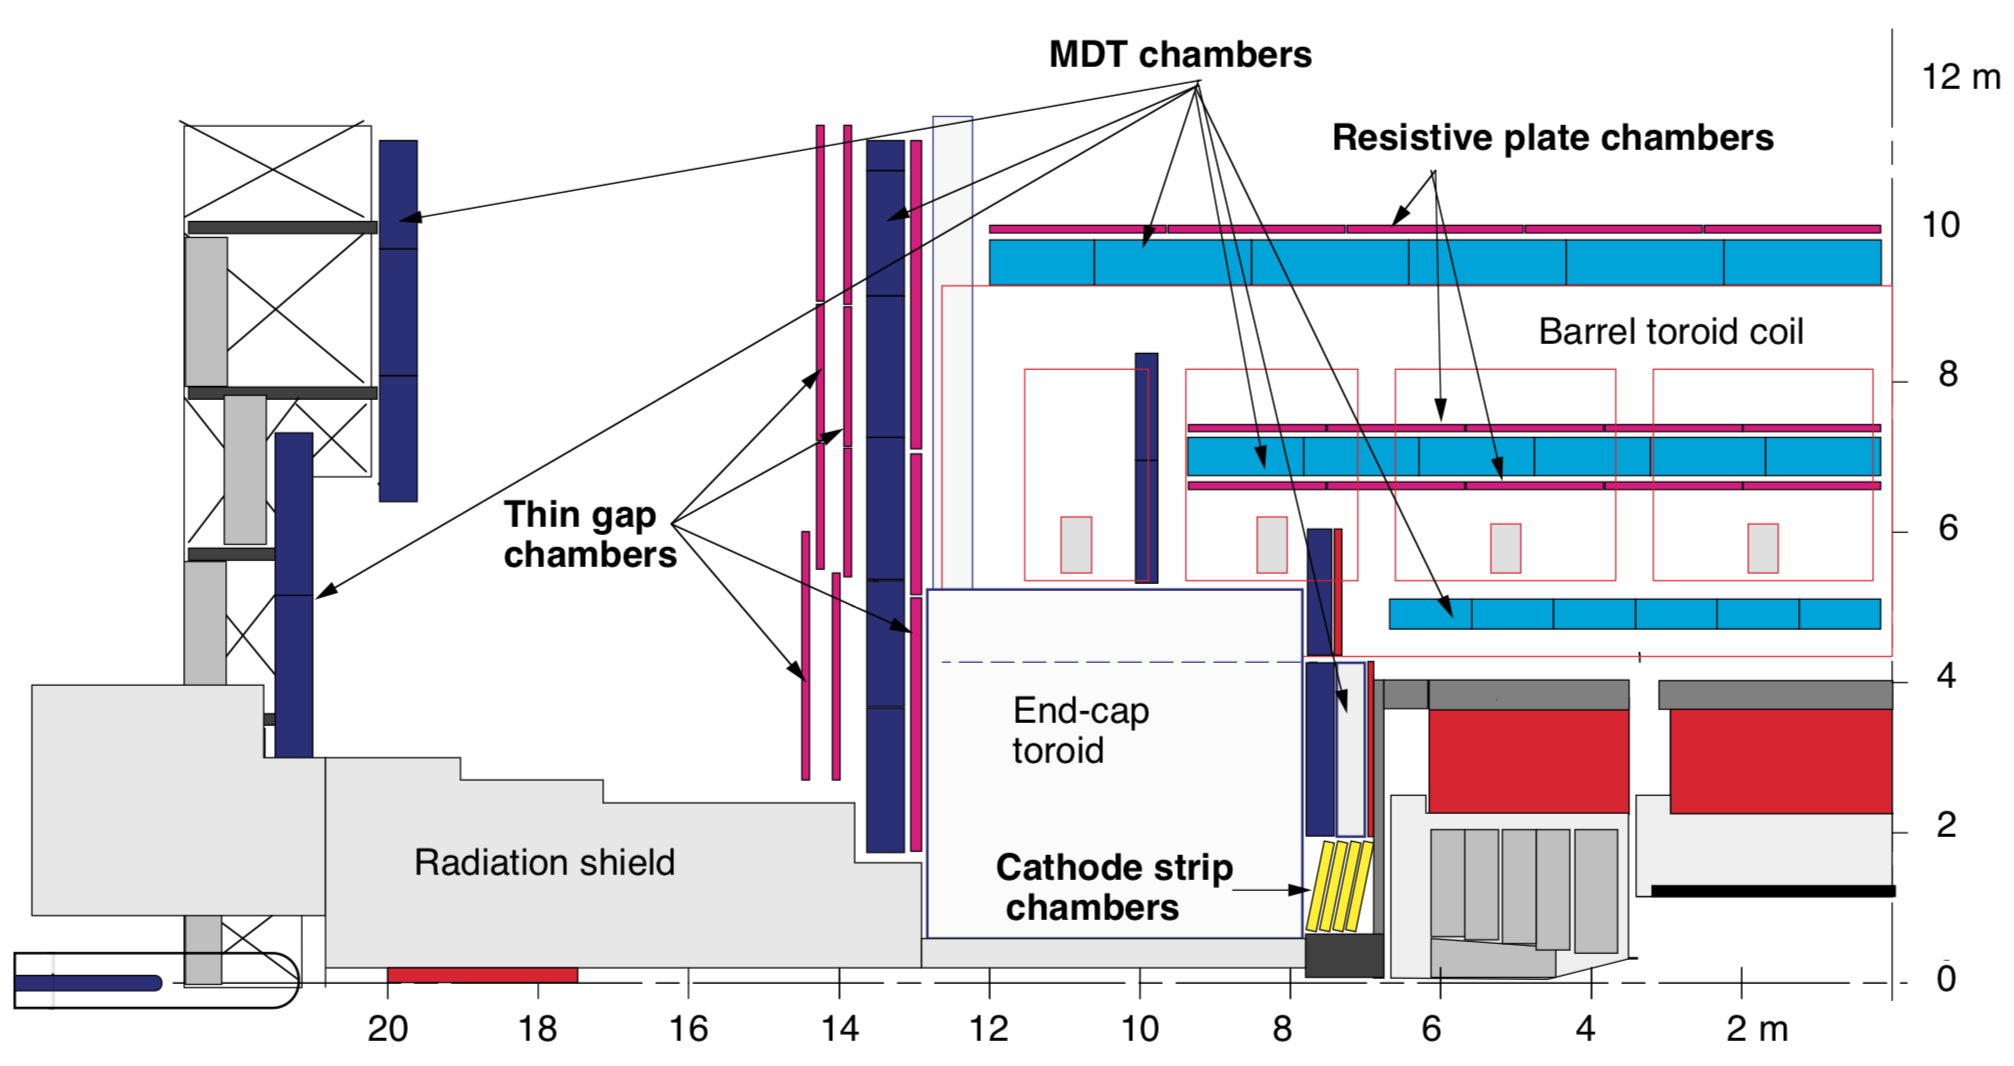
\includegraphics[width=\textwidth,keepaspectratio]{muon_side.png}
			\caption[Side view]{Side view}
			\label{fig::side}
		\end{subfigure}
		\hfill
		\begin{subfigure}[t]{0.33\textwidth} 
			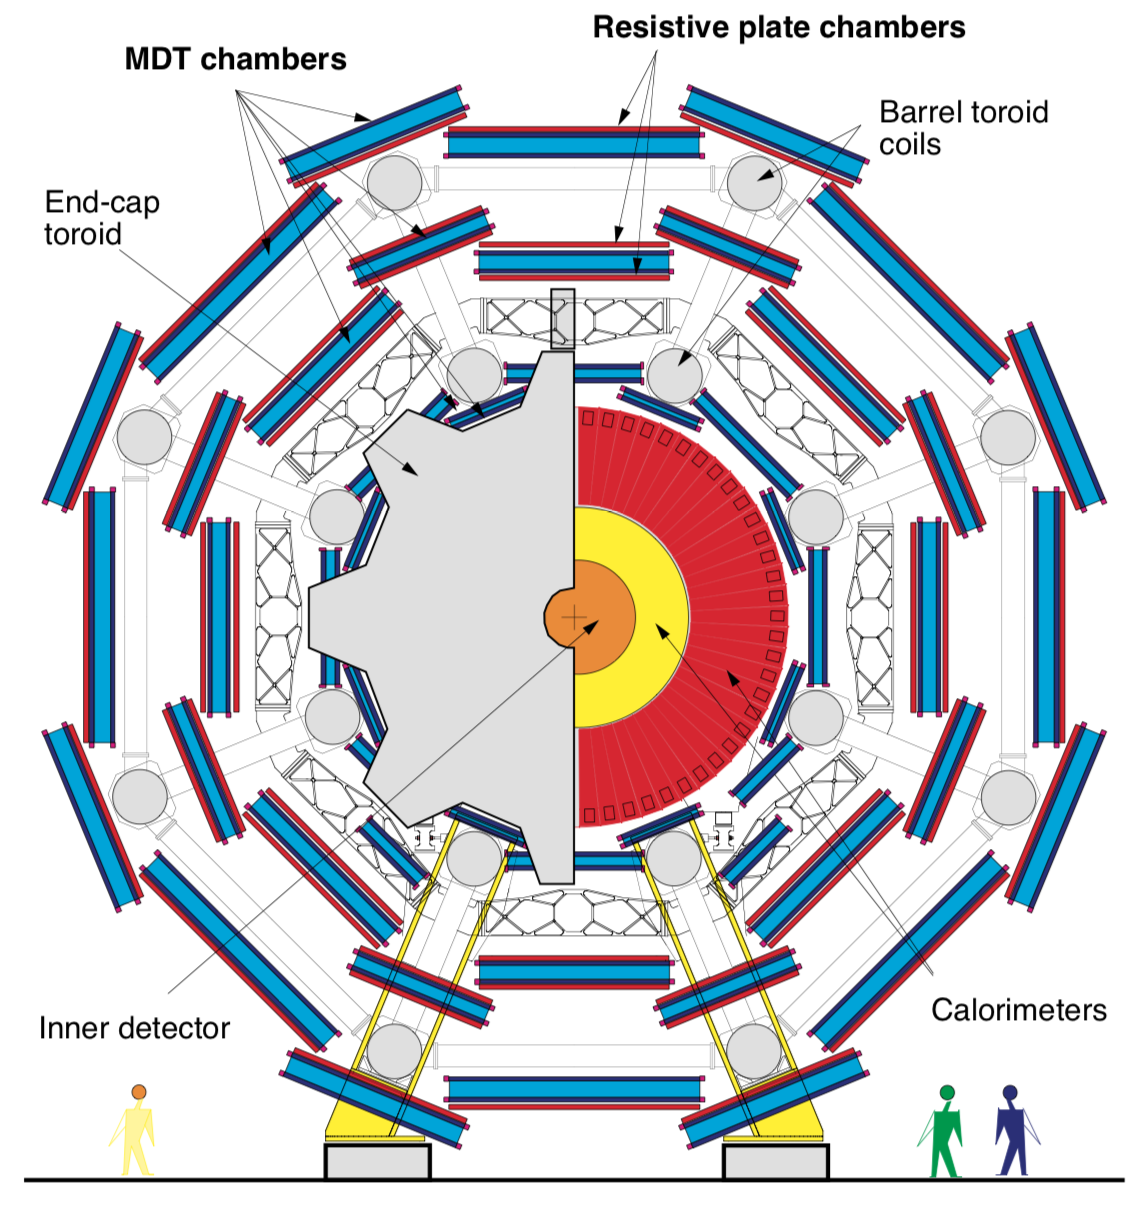
\includegraphics[width=\textwidth,keepaspectratio]{muon_trans.png}
			\caption[Tranverse view]{Tranverse view}
			\label{fig::transverse}
		\end{subfigure}
		\caption{Cut views of the muon systems}
		\label{fig::muon_cut}
	\end{figure}
	
	\begin{table}
	\centering
	\begin{tabular}{|l|c|}
		\hline	
		\textbf{Monitored drift tubes} & \textbf{MDT} \\
		Coverage & $|\eta| < 2.7$ (innermost layer: $|\eta| < 2.0$) \\
		Number of chambers  & 1088 (1050)\\
		Number of channels  & 339 000 (354 000)\\
		Function  & Precision tracking\\
		\hline	
		\textbf{Cathode strip chambers} & \textbf{CSC} \\
		Coverage & $2.0 < |\eta| < 2.7$  \\
		Number of chambers  & 32\\
		Number of channels  & 31 000\\
		Function  & Precision tracking\\
		\hline	
		\textbf{Resistive plate chambers} & \textbf{RPC} \\
		Coverage & $|\eta| < 1.05$  \\
		Number of chambers  & 544 (606)\\
		Number of channels  & 359 000 (373 000)\\
		Function  & Triggering, second coordinate\\
		\hline	
		\textbf{Thin gap chambers} & \textbf{TGC} \\
		Coverage & $1.05 < |\eta| < 2.7$  \\
		Number of chambers  & 3588\\
		Number of channels  & 318 000\\
		Function  & Triggering, second coordinate\\
		\hline	
	\end{tabular}\\
	\caption{ \gls{atlas} muon spectrometer subsystems coverage and parameters}
	\label{tab::muon_table}
\end{table}

\section{Forward detectors}
	There are three detector systems that cover the ATLAS forward region (see fig. \ref{fig::forward}): \gls{lucid}, \gls{alfa} and \gls{zdc}. The measurement of luminosity if the main goal of the first two detectors and has fundamental importance: it provides the normalization scale for all the observed processes.\\
	 \gls{lucid}\cite{lucid_1}, \cite{lucid_2} is the main \gls{atlas} relative luminosity monitor. The main purpose of the \gls{lucid} detector is to detect inelastic p-p scattering in the forward region measuring the integrated luminosity and performing online monitoring of the instantenous luminosity and beam conditions with uncertainty of about few percent. It is symmetrically installed at $\pm$17 m from the interaction point and at a radial distance of about 10 cm from the beam line (resulting in $|\eta| \approx 5.8$). On each side four bundles of quartz fibers are used as a medium producing Cherenkov radiation directing the Cherenkov light into the 16 \glspl{pmt} placed outside the radiation shielding. \\
	 The \gls{alfa}\cite{alfa} detector is used to measure the absolute luminosity through elastic scattering at small angles. In order to perform such measurement we need to meet the following conditions: \\
	 \begin{itemize} 
	\item  The beam has to be more parallel than normally. Special collider beam optics allowing high values of the amplitude function at the interaction point $\beta*$ together with reduced beam emittance. 
	\item  To be sensitive to small angles the detectors have to be placed as far as possible from the interaction point and close to the beam. This is why the detectors are located inside the Roman pots at $\pm$240 from the interaction point. On each side there are two Roman pots separared by four meters.
 	\end{itemize}
 	The Roman pot windows allow the elastically scattered protons reach the square scintillating fibres of 0.5 mm width which are in turn connected to multi-anode \glspl{pmt} through the light-guides. The detector provides a spacial resolution of 30 $\mu$m and allows to measure absolute luminosity with uncertainty of 1.7\% for the Run 2\cite{luminosity}. \\
	 \gls{zdc} are used to detect forward neutrons at $|\eta| > 8.3$ in heavy-ion collisions, which in turn allows to determine the centrality of such collisions.  The detector is installed at $\pm$140 m from the interaction point. Every \gls{zdc} arm consists of 4 modules: one electromagnetic and three hadronic. These modules are quartz rods shielded by the tungsten plates and connected to the \glspl{pmt} via the light-guides allowing to measure incending particle energy and position. The EM module has a better position resolution mapping each of 96 quartz rods into a single pixel, while the hadronic modules map a bundle of four rods into a pixel. Only one of the three hadronic modules per arm provide position-sensing rods and only the arm at -140 m has the position-sensing EM module.  
    \begin{figure}[htpb]
	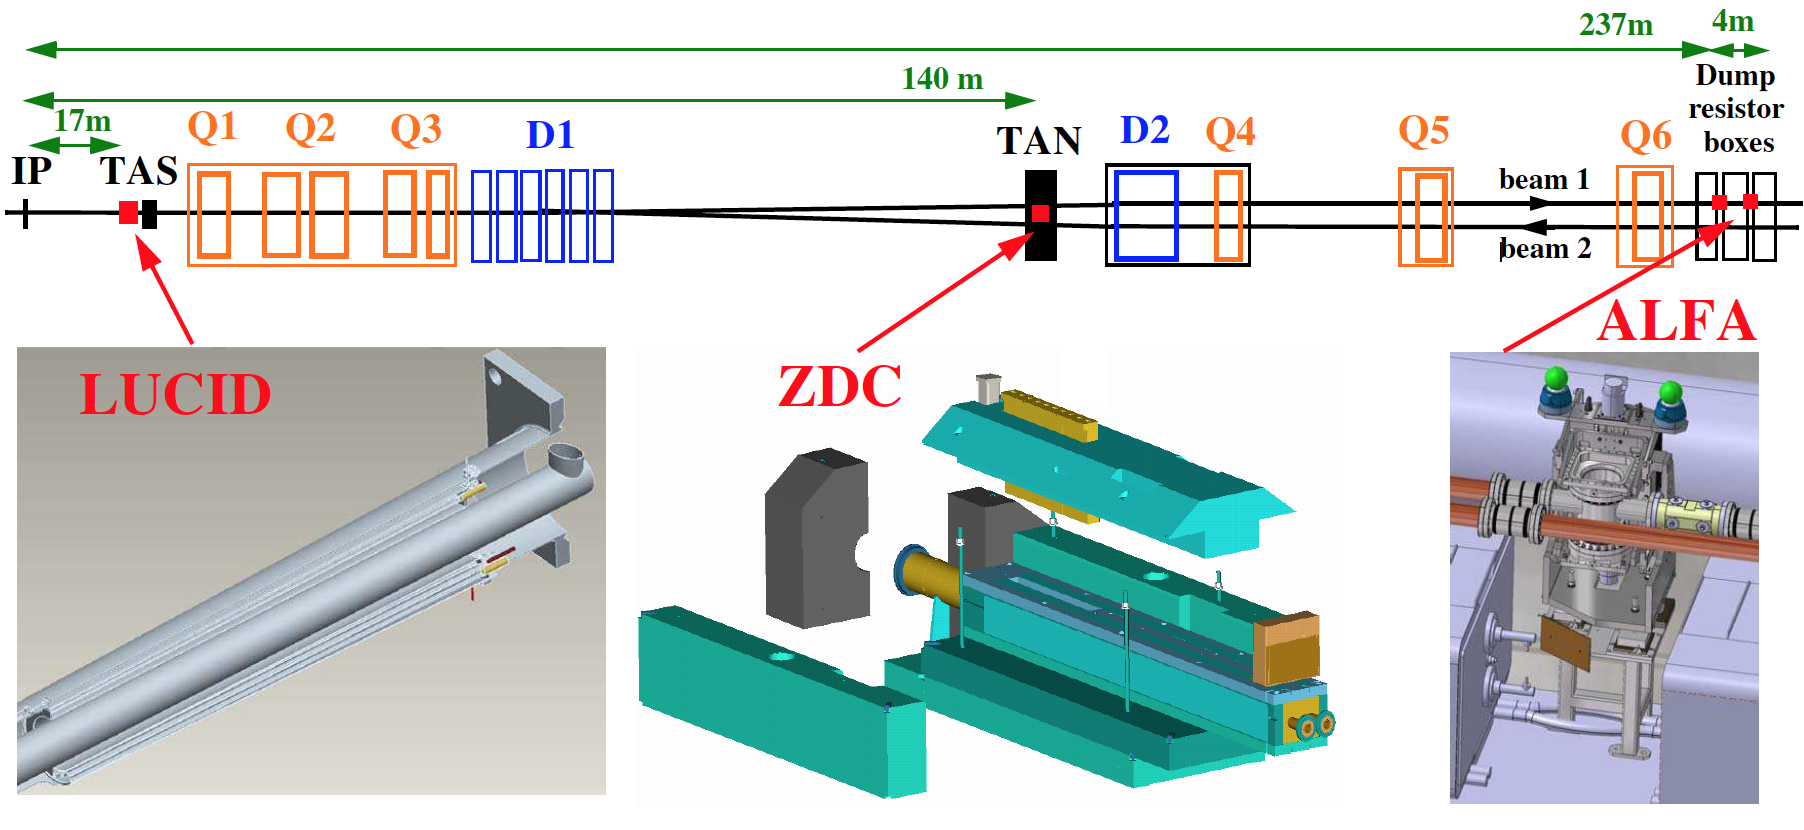
\includegraphics[width=\textwidth,keepaspectratio]{forward.png}
	\caption{ \gls{atlas} forward detectors}
	\label{fig::forward}
\end{figure}
\section{Trigger system}
\label{sect::trigger}
 Considering that the bunch crossing rate at LHC is about 40 MHz and that \gls{atlas} detector has over one million read-out channels it would never be possible to store all the raw data without significant preselection that would decrease the data rate. The selection criteria are picked to retain and store only the events which might be interesting for the LHC physics. The preselection and storage is conducted with the help of \gls{tdaq} systems. \\
 The trigger system has three distincs levels: L1, L2 and the event filter,  the two latter levels are also called \gls{hlt}. Each next level refines the decisions made before and, if necessary, applies additional selection, further lowering the event rate. The data acquisition system receives and buffers the event data from the readout electronics at the L1 trigger accept rate which for Run 2 is about 100 kHz \cite{daq}. The \gls{hlt} then lowers the rate down to 1.5 kHz which is then stored for the offline analysis. \\
 The L1 trigger looks for muons, electrons, photons, jets at handrons from $\tau$-lepton decays with high transverse momentum, large missing and total transverse energy. The muons of interest are identified using the muon spectrometer trigger system described in section \ref{sect::muons}. The rest of the particles are selected using the information from all the calorimeters with reduced granularity.  During the Run 2 an intermediate L1Topo trigger was also added allowing to combine the information from the spectrometer and calorimeter and extend possible trigger selections. Results from these triggers gets processed by the central trigger processor which implements the trigger menu made up of different combinations of trigger selections. The decision latency for the L1 trigger must not exceed 2.5 $\mu$s after the corresponding bunch crossing. \\
 For every selected event the L1 defines one or more regions called \gls{roi} which include the $\eta$ and $\phi$ coordinates of these regions for their subsequent use by the \gls{hlt}. The L2 selection is seeded \gls{roi} and uses full grnularity and precision along with other detector data available. The trigger block diagram is presented in fig. \ref{fig::trigger}.
    \begin{figure}[htpb]
	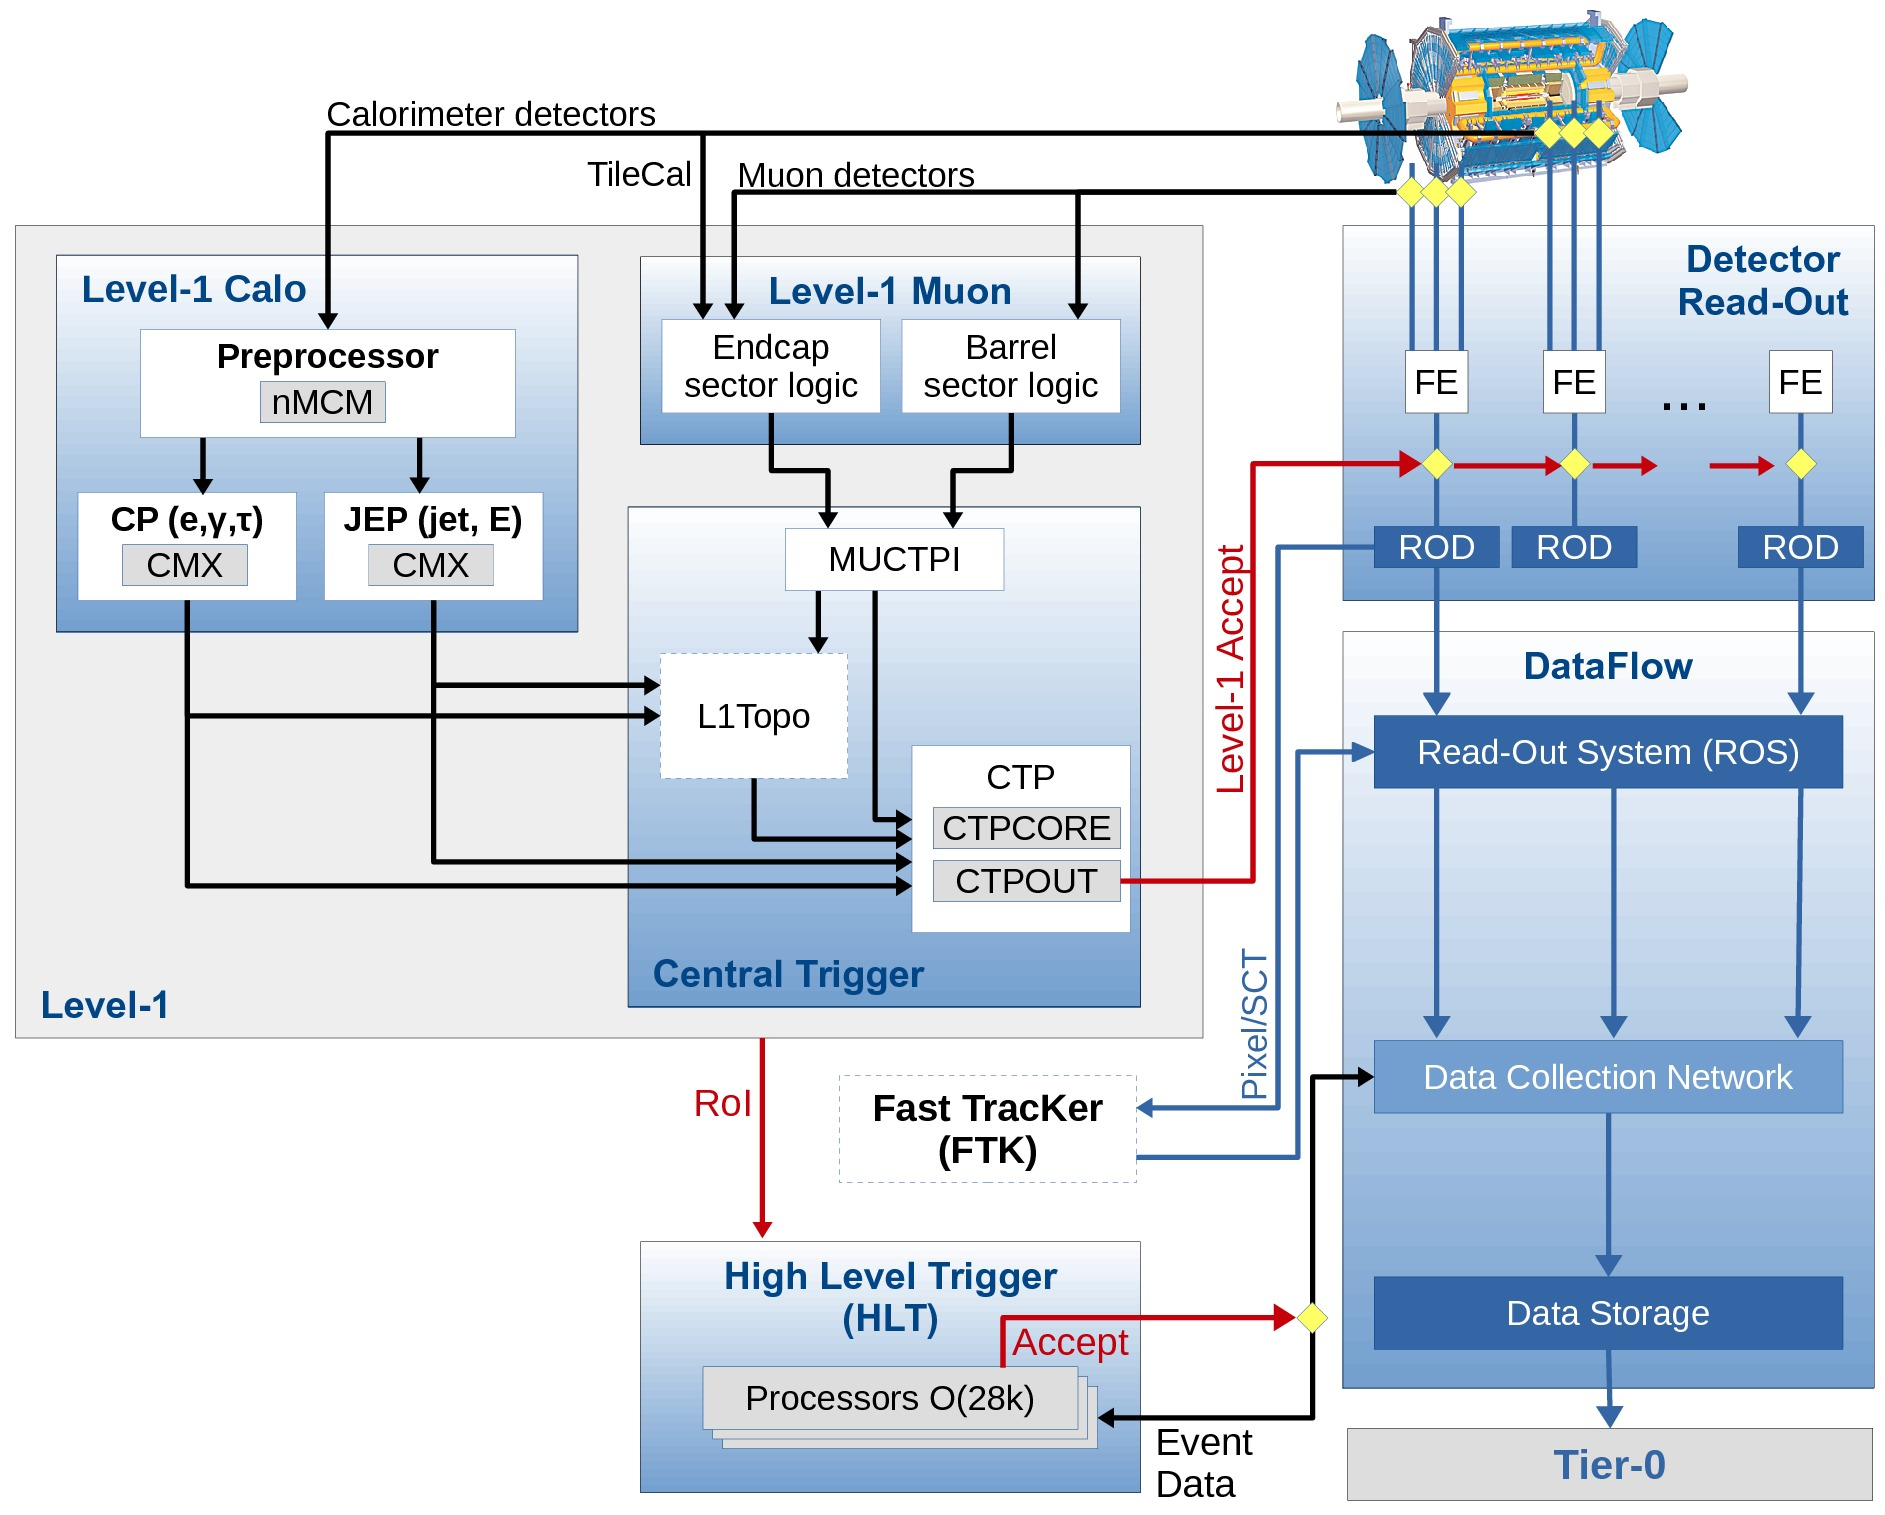
\includegraphics[width=\textwidth,keepaspectratio]{trigger.jpg}
	\caption{ The scheme of \gls{atlas} trigger systems}
	\label{fig::trigger}
\end{figure}